\section{Experiments}
\label{sec:results}

\subsection{Experimental Setting}
% Dataset and evaluation metrics

To conduct experiments for our proposed methods, datasets FB15K-237, which is a variant of FB15K \cite{bollacker2008freebase}, as well as WN18 \cite{miller1995wordnet} are used. For evaluation, our results will be achieved by training the TransE, DistMult, and RotatE models, during which the train set triplets consist of positive triplets $(h , r, t)$ as well as negative triplets, $(h', r, t')$. To evaluate the impact of our NEG schemes on the learned embedding, Hits at N (H@N),  Mean Rank (MR), and Mean Reciprocal Rank (MRR) are used as evaluation measures. 

% Hyperparameter and baseline

For the negative sampling step, $k$ is the main hyperparameter which determines the \emph{k-hop} neighbourhood of each entity. 
% ------------------------------------------------------
% Remove start
\cut{
Furthermore, another important hyperparameter in our scheme is the number of random walks, denoted as $\omega$, when \emph{Random Walks} is being used to approximate the \emph{k-hop} neighbourhood. }
% Remove end
% ------------------------------------------------------

Lastly, our baselines are the results achieved after training the same graph embedding model combined with uniform NEG, and Self-Adversarial NEG, as done in \cite{sun2019rotate}. The hyperparameters that yield the best performance of graph embedding models on the validation set can be found in Section \ref{sec:supplemental}.

\subsection{Results}

% Our most important findings
    % we beat uniform baseline 
    % we need 3500 RW to approximate the adjacency tensor 
    % our matrices are sparse according to table 3
    % We observe that a relatively small subset of nodes ---i.e. 26%, are needed to achieve competitive performance with SOTA methods reaffirming our original hypothesis local negatives in KG's provide a useful learning signal.

\cut{
To infer the number of random walks which can adequately approximate the k-hop tensor, we investigated the effect of different numbers of random walks, $\omega$, ranging from 100 to 3000 illustrated in Figure \ref{fig:ablation}. In these graphs, two baselines are exhibited, namely the one representing the output when negative sampling was done uniformly, and the other being our best performance achieved by our Uniform SANS combined with TransE, for which the k-hop tensor was explicitly computed. According to our observations, our model beats both baselines when the k-hop tensor is approximated with 3000 random walks. This result can be justified by acknowledging that the nodes’ indices that are within close proximity in the k-hop tensor will have larger values; this will yield a weighted negative sampling scheme and may be the contributor to the increased performance.

\begin{figure}[h]
    \centering
    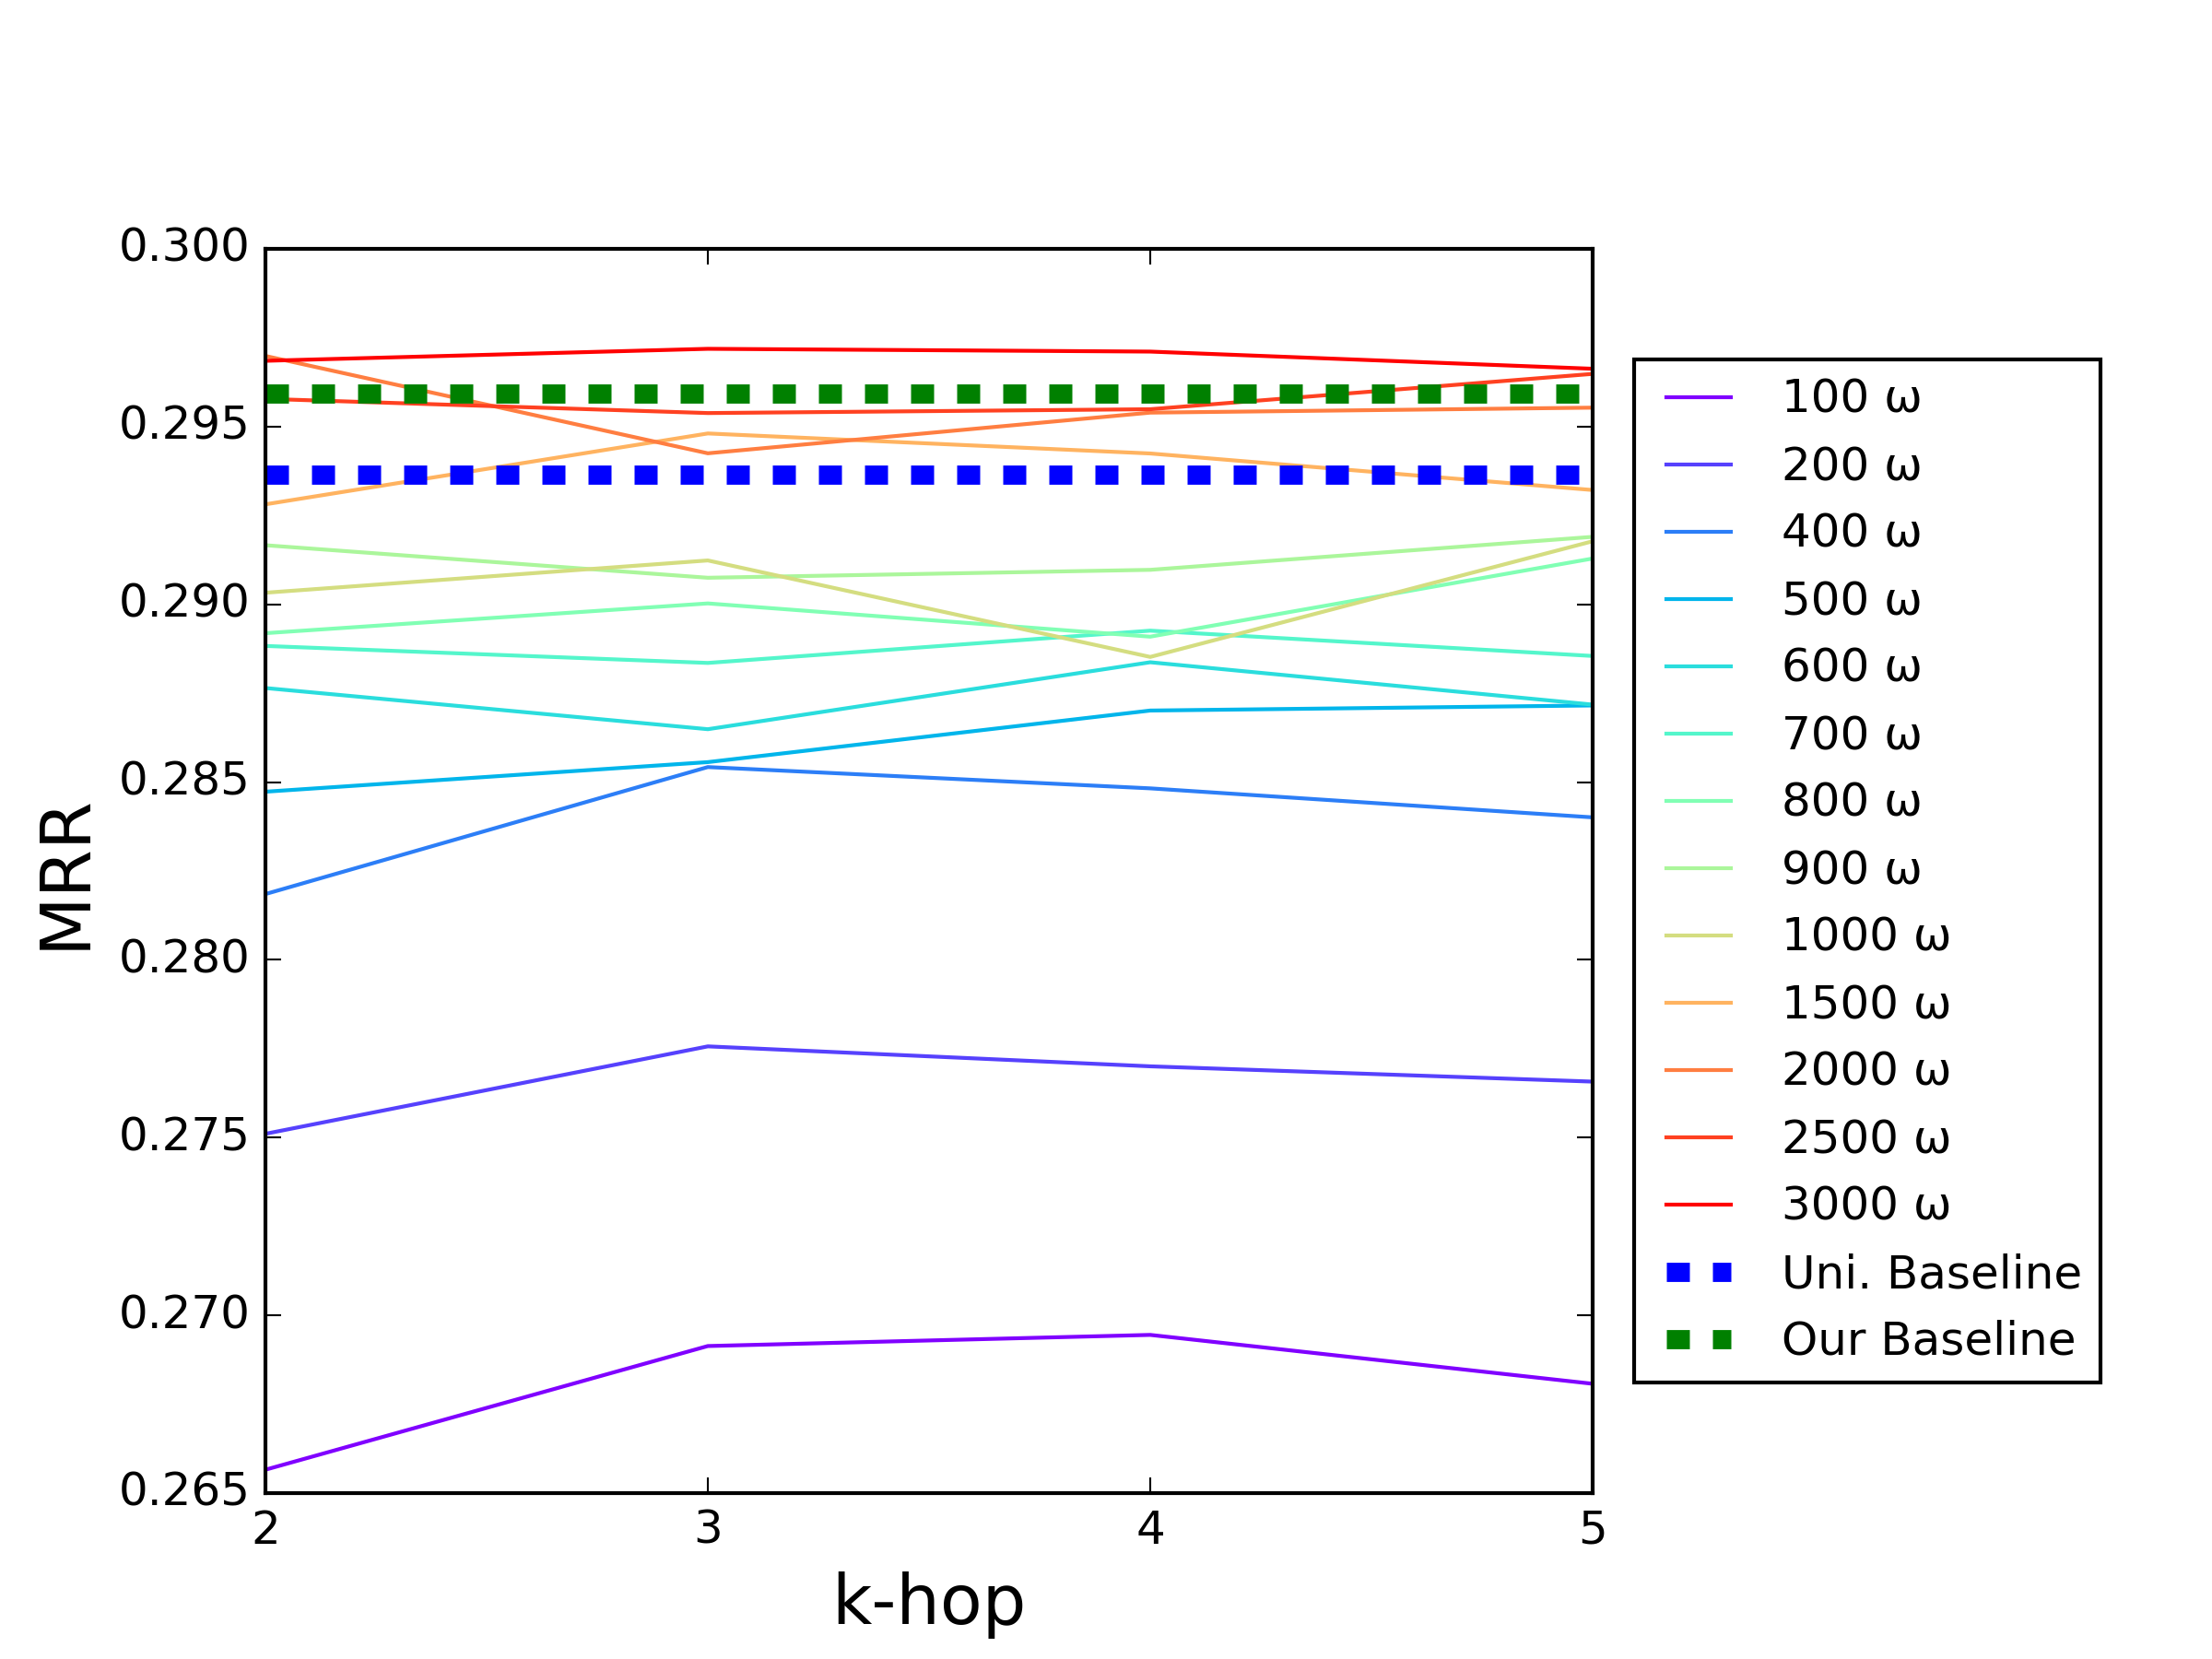
\includegraphics[width=2.5in]{writeup/Results/Ablation.png}
    \caption{The effect of the number of random walks
     for Uniform SANS with the TransE on FB 15k-237.}
    \label{fig:ablation}
\end{figure}
}
% ------------------------------------------------------------------------
% MAIN RESULTS TABLE START

\begin{table*}[h]
\begin{small}
\centering
\begin{tabular}{cccccccc}
\hline
\multirow{3}{2cm}{\centering Score Function}& \multirow{3}{2cm}{Algorithm} & \multicolumn{2}{c}{FB15K-237} & \multicolumn{2}{c}{WN18} & \multicolumn{2}{c}{WN18RR} \\
& & Hit@10 & \multirow{2}{1cm}{\centering MRR} & Hit@10 & \multirow{2}{1cm}{\centering MRR} & Hit@10 & \multirow{2}{1cm}{\centering MRR} \\ 
& & (\%) & & (\%) & & (\%) & \\
\hline
% TransE --------------------------------------------------
\multirow{5}{1.5cm}{\centering TransE} & Uniform \cite{sun2019rotate} & 48.03 & 0.2927 & \textbf{95.53} & 0.6085 & 49.63 & 0.2022 \\
& KBGAN \cite{cai2017kbgan} & 46.59 & 0.2926 & 94.80 & 0.6606 & 45.39 & 0.1808 \\
& IGAN \cite{wang2018incorporating} & - & - & 92.7 & - & - & -\\
& NSCaching \cite{zhang2019nscaching} & 47.64 & 0.2993 & 94.63 & 0.7818$^\dagger$ & 47.83 & 0.2002\\
& Self-Adv. \cite{sun2019rotate} & \textbf{52.73} & \textbf{0.3296} & 92.02 & 0.7722 & 52.78 & 0.2232 \\
& Uniform SANS (ours) & 48.73 & 0.2971 & 95.22$^\dagger$ & \textbf{0.8195} \\
& Self-Adv. SANS (ours) & 50.04$^\dagger$ & 0.3060$^\dagger$ & 88.51 & 0.7429 \\
\hline
% DistMult --------------------------------------------------
\multirow{4}{1.5cm}{\centering DistMult} & Uniform & 40.26 & 0.2537 & 81.39  & 0.4689 & 52.86 & 0.3938 \\
& KBGAN & 39.91 & 0.2272 & 93.08$^\dagger$ & 0.7275$^\dagger$ & 44.32 & 0.3849 \\
& NSCaching & 45.56 & 0.2834 & \textbf{93.74} & \textbf{0.8306} & 45.80 & 0.4148\\
& Self-Adv. & \textbf{48.41} & \textbf{0.3091} & 92.94  & 0.6837 & 53.80 & 0.4399 \\
& Uniform SANS (ours) & 41.46 & 0.2621 & 89.80 & 0.6234 \\
& Self-Adv. SANS (ours) & 48.07$^\dagger$ & 0.3058$^\dagger$ & 91.08  & 0.6633 \\
\hline
% RotatE --------------------------------------------------
\multirow{3}{1cm}{\centering RotatE} & Uniform & 47.85 & 0.2946 & \textbf{96.09} & 0.9474 & 56.51 & 0.4711 \\
& Self-Adv. & \textbf{53.03} & \textbf{0.3362} & 96.05$^\dagger$ & \textbf{0.9498} & 57.29 & 0.4760 \\
& Uniform SANS (ours) & 48.47 & 0.3003 & \textbf{96.09} & 0.9496$^\dagger$ \\
& Self-Adv. SANS (ours) & 51.07$^\dagger$ & 0.3161$^\dagger$ & 96.05$^\dagger$ & \textbf{0.9498} \\
\hline
\end{tabular}
\caption{Comparison of different negative sampling algorithms. Results for KBGAN and NSCaching are taken from \cite{zhang2019nscaching}. IGAN results are taken from \cite{wang2018incorporating}. 
All other results were are taken from our re-implementations. Bold numbers are the best performance, whereas those marked by $\dagger$ are the second-best. 
}
\label{tab:comparison}
\end{small}
\end{table*}

% MAIN RESULTS TABLE END
% ------------------------------------------------------------------------

% % % ------------------------------------------------------------------------
% % of filled entries
\begin{table}[b]
\centering
\begin{tabular}{cccccc}
\hline
$k$ & 2 & 3 & 4 & 5 \\ 
\hline
FB15K-237 & 34 & 83 & 97 & 99 \\
\hline
WN18 & 0.19 & 0.75 & 3.22 & 10.2 \\
\hline
WN18RR & - & - & - & - \\
\hline
\end{tabular}
\caption{Percentage (\%) of the k-hop adjacency tensor that is filled.}
\label{tab:percentage}
\end{table}
% % % ------------------------------------------------------------------------

Table \ref{tab:comparison} is indicative of the best performances achieved while deploying different negative sampling algorithms to train different graph embedding models. As seen, our Uniform SANS performs better than uniform sampling by constraining negative sampling to the \emph{k-hop} neighbourhood. Moreover, our Self-Adversarial SANS performs better than GAN-based and cache-based methods, and exhibits similar performance to the Self-Adversarial technique proposed in \cite{sun2019rotate}. Therefore, our experimental findings suggest that both of our negative sampling algorithms are simple yet effective NEG techniques, with comparable performances to the state-of-the-arts. Most notably, our NEG algorithms require less computational resources for using a smaller distribution of negative triplets. This is verified by Table \ref{tab:percentage}, where the percentage of filled entries in the \emph{k-hop} adjacency tensor have been listed. 

Lastly, comparing the results obtained with our Uniform SANS scheme to the ones achieved by NSCaching, which uses high quality negative triplets, indicated that nodes within close proximity to each other may create ``hard'' negative examples, which supports our initial hypothesis. A more detailed set of experimental findings, presenting the performance of our negative sampling algorithms against uniform sampling and self-adversarial sampling with different hyperparameters, as well as information regarding their space and time complexity can be found in \ref{sec:supplemental}.

% --------------------------------------------------------------------------------------------------------------------

\cut{
Additionally, Table \ref{tab:times} compares the time and space complexity of different NEG algorithms, which emphasize the cheapness of their runtime and space complexities compare to the state-of-the-arts. 

Lastly, Table \ref{tab:percentage} also shows the percentage of filled entries in the \emph{k-hop} adjacency matrix, that is informative of the size of the subspace from which negative examples are drawn from. With regards to these values, our NEG algorithm uses a smaller negative sampling subspace compared to the standard NEG approaches, yet demonstrates comparable performance. A more detailed set of results, presenting the performance of our NEG algorithms against uniform sampling and self-adversarial sampling with different hyperparameters, can be found in our supplementary document.
}
